\section{String Matching}

\subsection{The naive string-matching algorithm}

\begin{description}
\descitem{32.1-1} \textit{Show the comparisons the naive string matcher makes for the pattern $P = 0001
$ in the text $T = 000010001010001$.}

\begin{ex}
    \begin{figure}[H]
      \centering
      \begin{subfigure}[t]{.45\textwidth}
        \centering
        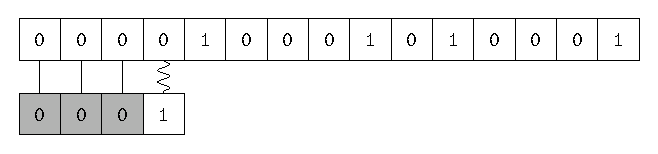
\includegraphics[scale=.6]{img/32_1-1/32_1-1_1.pdf}
        \caption{$\texttt{shift} = 0$}\label{fig:32_1-1_1}
      \end{subfigure}
      \begin{subfigure}[t]{.45\textwidth}
        \centering
        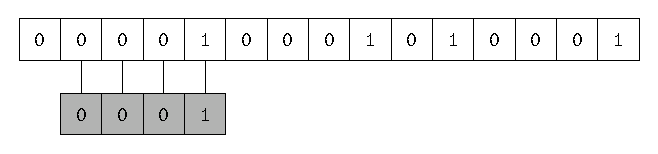
\includegraphics[scale=.6]{img/32_1-1/32_1-1_2.pdf}
        \caption{$\texttt{shift} = 1$}\label{fig:32_1-1_2}
      \end{subfigure}
      \begin{subfigure}[t]{.45\textwidth}
        \centering
        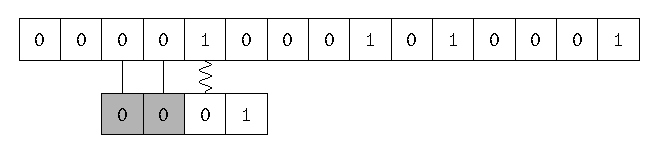
\includegraphics[scale=.6]{img/32_1-1/32_1-1_3.pdf}
        \caption{$\texttt{shift} = 2$}\label{fig:32_1-1_3}
      \end{subfigure}
      \begin{subfigure}[t]{.45\textwidth}
        \centering
        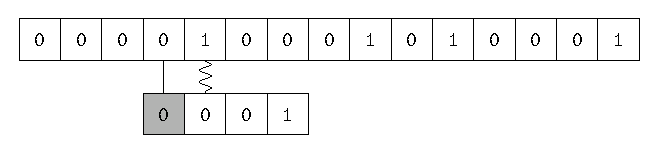
\includegraphics[scale=.6]{img/32_1-1/32_1-1_4.pdf}
        \caption{$\texttt{shift} = 3$}\label{fig:32_1-1_4}
      \end{subfigure}
      \begin{subfigure}[t]{.45\textwidth}
        \centering
        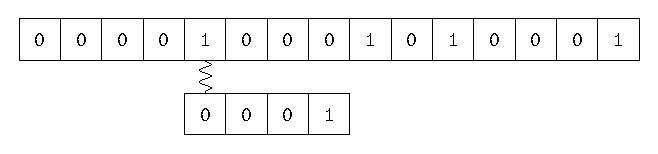
\includegraphics[scale=.6]{img/32_1-1/32_1-1_5.pdf}
        \caption{$\texttt{shift} = 4$}\label{fig:32_1-1_5}
      \end{subfigure}
      \begin{subfigure}[t]{.45\textwidth}
        \centering
        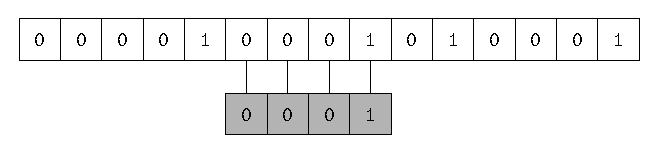
\includegraphics[scale=.6]{img/32_1-1/32_1-1_6.pdf}
        \caption{$\texttt{shift} = 5$}\label{fig:32_1-1_6}
      \end{subfigure}
      \begin{subfigure}[t]{.45\textwidth}
        \centering
        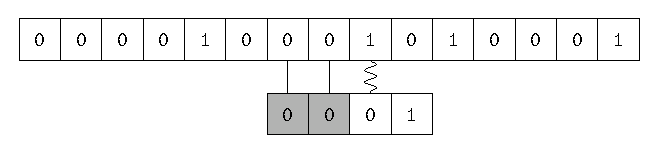
\includegraphics[scale=.6]{img/32_1-1/32_1-1_7.pdf}
        \caption{$\texttt{shift} = 6$}\label{fig:32_1-1_7}
      \end{subfigure}
      \begin{subfigure}[t]{.45\textwidth}
        \centering
        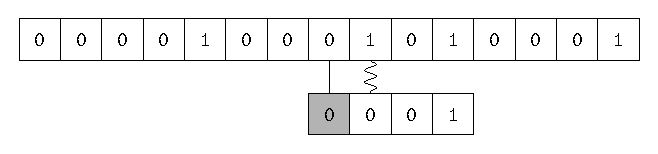
\includegraphics[scale=.6]{img/32_1-1/32_1-1_8.pdf}
        \caption{$\texttt{shift} = 7$}\label{fig:32_1-1_8}
      \end{subfigure}
      \begin{subfigure}[t]{.45\textwidth}
        \centering
        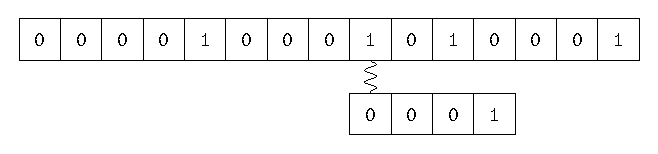
\includegraphics[scale=.6]{img/32_1-1/32_1-1_9.pdf}
        \caption{$\texttt{shift} = 8$}\label{fig:32_1-1_9}
      \end{subfigure}
      \begin{subfigure}[t]{.45\textwidth}
        \centering
        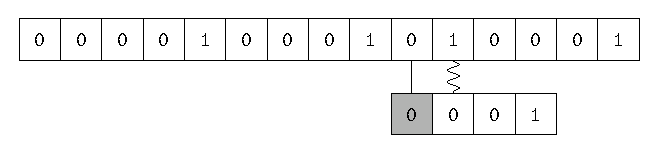
\includegraphics[scale=.6]{img/32_1-1/32_1-1_10.pdf}
        \caption{$\texttt{shift} = 9$}\label{fig:32_1-1_10}
      \end{subfigure}
      \begin{subfigure}[t]{.45\textwidth}
        \centering
        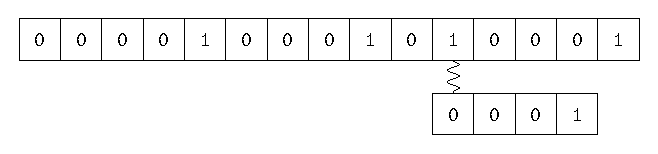
\includegraphics[scale=.6]{img/32_1-1/32_1-1_11.pdf}
        \caption{$\texttt{shift} = 10$}\label{fig:32_1-1_11}
      \end{subfigure}
      \begin{subfigure}[t]{.45\textwidth}
        \centering
        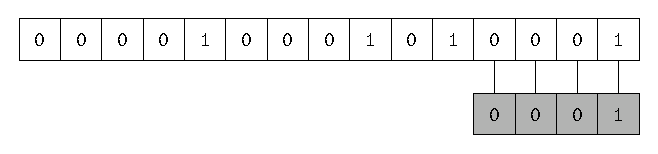
\includegraphics[scale=.6]{img/32_1-1/32_1-1_12.pdf}
        \caption{$\texttt{shift} = 11$}\label{fig:32_1-1_12}
      \end{subfigure}
      \caption{Recherche de la sous châine $0001$ dans $000010001010001$ avec l'algorithme naïve.} 
      \label{fig:naive-match-string} 
    \end{figure}
\end{ex}


\descitem{32.1-2} \textit{Suppose that all characters in the pattern $P$ are different. Show how to accelerate
\proc{Naive-String-Matcher} to run in time $O(n)$ on an $n$-character text $T$.}

\begin{ex}
\begin{codebox}
\Procname{\algo{Naive-String-Matcher-Diff}$(\id{T}, \id{P})$}
    \li $n = \attrib{T}{length}$
    \li $m = \attrib{P}{length}$
    \li $s = 0$
    \li \While $\id{s} <= n -m$ \Do
    \li \If $P[1\twodots m] == T[s + 1\twodots s + m]$ \Then
    \li print "Pattern occurs with shift" s 
    \li $s \gets s + 1$ 
    \li \Else 
    \li $s \gets s + m$ \End
\end{codebox}
\end{ex}

\descitem{32.1-3} \textit{}
\descitem{32.1-4} \textit{Suppose we allow the pattern $P$ to contain occurrences of a gap character $\diamondsuit$ that
can match an \textit{arbitrary} string of characters (even one of zero length). For example,
the pattern $ab\diamondsuit ba\diamondsuit c$ occurs in the text $cabccbacbacab$ abstract as}

    $c\smallunderbrace{ab}_{ab}\smallunderbrace{cc}_{\diamondsuit}\smallunderbrace{ba}_{ba}\smallunderbrace{cba}_{\diamondsuit}\smallunderbrace{c}_{c}ab$

\textit{and as}

    $c\smallunderbrace{ab}_{ab}\smallunderbrace{ccbac}_{\diamondsuit}\smallunderbrace{ba}_{ba}\smallunderbrace{}_{\diamondsuit}\smallunderbrace{c}_{c}ab$.

\begin{ex}

\begin{codebox}
\Procname{\algo{Naive-String-Matcher-With-Gap}$(\id{T}, \id{P}, \id{gap})$}
    \li $n = \attrib{T}{length}$,  $m = \attrib{P}{length}$, $s = 0$, $\id{flag} = \const{true}$
    \li \For each $P_i$ in partition $P$ delimited by $\id{gap}$ character \Do
    \li $m_i = \attrib{P_i}{length}$
    \li \While $s <= n - m$ \Do
    \li \If $P_i[1\twodots m_i] == T[s + 1\twodots s + m_i]$ \Then
    \li \If $\id{\id{flag}}$ \Then
    \li $\id{shift} \gets s$
    \li $\id{flag} \gets \const{false}$ \End
    \li \textbf{break}
    \li \Else 
    \li $s \gets s + 1$ \End \End \End
    \li \If $s <= n-m$ \Then
    \li print "Pattern occurs with shift" \id{shift} \End
\end{codebox}
\end{ex}

\end{description}

\subsection{The Rabin-Karp algorithm}

\begin{description}
\descitem{32.2-1} \textit{Working modulo $q = 11$, how many spurious hits does the Rabin-Karp matcher encounter in the text $T = 3141592653589793$ when looking for the pattern $P = 26$?}
\begin{ex}
Trois, car $26 \equiv 15 \equiv 59 \equiv 92\mod 11$.
\end{ex}
\descitem{32.2-2} \textit{}
\descitem{32.2-3} \textit{}
\descitem{32.2-4} \textit{}
\end{description}

